%%%%%%%%%%%%%%%%%%%%%%%%%%%%%%%%%%%%%%%%%%%%%%%%%%%%%%%%%%%%%%%%%%%%%%
% Modelo artigo SBC
% Disponível em:
% https://www.sbc.org.br/documentosinstitucionais/#publicacoes
% https://www.overleaf.com/latex/templates/sbc-conferences-template-updated-sbc-template-dot-sty-v2017/pyhttxftxjqn
%%%%%%%%%%%%%%%%%%%%%%%%%%%%%%%%%%%%%%%%%%%%%%%%%%%%%%%%%%%%%%%%%%%%%%

\documentclass[12pt]{article}

\usepackage{sbc-template}
\usepackage{graphicx,url}
\usepackage[utf8]{inputenc}
\usepackage[brazil]{babel}

% --- Adicionado esta linha abaixo para remover o número 1 antes do endreço
\def\instnum{} 
     
\sloppy

\title{Instructions for Authors of SBC Conferences\\ Papers and Abstracts}

\author{Ana Paula dos Reis Barreto, João Antonio Silveira Matos}

\address{Pós-Graduação --  Universidade Tiradentes (UNIT)\\
  Aracaju, SE -- Brazil
  \email{ana.reis@souunit.com.br, joao.asilveira@souunit.com.br}}


\begin{document} 

\maketitle

\begin{abstract}
This paper presents a comparative study using machine learning techniques to predict and classify the academic performance of undergraduate students in Brazil, utilizing historical data from the National Exam of Student Performance (ENADE) spanning from 2008 to 2018. To handle the massive dataset (over 3.7 million records) and high class imbalance, the continuous final score was categorized into three performance ranges (unsatisfactory, adequate, and high). A robust preprocessing pipeline was applied, consisting of One-Hot Encoding for categorical variables, scaling by StandardScaler, and majority class downsampling. Three classification algorithms were evaluated: Decision Tree, Naive Bayes, and K-Nearest Neighbors (KNN). The results demonstrated that while simple models face generalization limits due to the high dimensionality of course and institutional variables, the KNN model achieved the best overall relative performance in identifying intermediate score categories (Macro F1-Score of 0.3976). The study concludes that socioeconomic factors and the field of study are the main driving vectors of student academic achievement.

\end{abstract}
     
\begin{resumo} 
Este trabalho apresenta um estudo comparativo utilizando técnicas de aprendizado de máquina para prever e classificar o desempenho acadêmico de estudantes de graduação no Brasil, utilizando dados históricos do Exame Nacional de Desempenho de Estudantes (ENADE) entre os anos de 2008 e 2018. Para lidar com o volume massivo de dados (mais de 3,7 milhões de registros) e o forte desbalanceamento de classes, a nota contínua foi categorizada em três faixas de rendimento (insatisfatório, adequado e elevado), sendo aplicado um pré-processamento robusto composto por codificação de variáveis categóricas via One-Hot Encoding, padronização (StandardScaler) e subamostragem (downsampling). Foram avaliados três algoritmos de classificação: Árvore de Decisão, Naive Bayes e K-Nearest Neighbors (KNN). Os resultados demonstraram que, embora modelos simples apresentem limitações de generalização decorrentes da alta dimensionalidade das variáveis de curso e instituição, o KNN obteve o melhor desempenho relativo na identificação de faixas intermediárias de notas (F1-Score Macro de 0,3976). O estudo aponta que fatores socioeconômicos e o tipo de curso são os principais vetores de influência no rendimento avaliado.
\end{resumo}


\section{Introdução}

A avaliação sistemática do Ensino Superior no Brasil, especialmente por meio do Exame Nacional de Desempenho de Estudantes (ENADE), constitui um importante instrumento para a formulação de políticas públicas e o monitoramento da qualidade da formação acadêmica. Entretanto, o grande volume de dados gerados pelo exame, que entre 2008 e 2018 reuniu informações de mais de 3,7 milhões de estudantes, apresenta desafios para a identificação de padrões associados ao desempenho discente. Nesse contexto, a Mineração de Dados Educacionais (Educational Data Mining – EDM) e o Aprendizado de Máquina (Machine Learning) oferecem recursos para a análise de grandes conjuntos de dados e o desenvolvimento de modelos preditivos. Contudo, fatores como o desbalanceamento das classes e a alta dimensionalidade das variáveis representam desafios para a construção desses modelos. Diante disso, este estudo tem como objetivo desenvolver e comparar modelos de classificação baseados nos algoritmos Árvore de Decisão, Naive Bayes e K-Nearest Neighbors (KNN), visando categorizar o desempenho dos estudantes em três níveis: insatisfatório, adequado e elevado. Adicionalmente, são investigadas estratégias de engenharia e seleção de atributos, incluindo a criação da variável `\texttt{tempo\_hiato}' e a utilização da importância de atributos baseada em florestas aleatórias, com o propósito de reduzir os efeitos da dimensionalidade e aprimorar o desempenho preditivo. A avaliação dos modelos é realizada por meio da métrica F1-Score, permitindo comparar sua capacidade de classificação e identificar abordagens mais adequadas à análise do desempenho acadêmico no contexto do ENADE.

\section{Metodologia} \label{sec:Mmtodologia}

Nesta seção, descreve-se a abordagem metodológica adotada para a modelagem preditiva das notas do ENADE. O fluxo de trabalho engloba desde a aquisição e pré-processamento dos dados até o balanceamento das classes, engenharia de atributos e a configuração experimental dos algoritmos de classificação.

\subsection{Base de Dados e Filtragem Temporal}

O conjunto de dados inicial provém do repositório histórico do ENADE (2008 a 2018), totalizando 3.712.412 registros e 20 atributos originais. Visando criar um cenário experimental mais próximo da realidade contemporânea do exame, o conjunto total de dados foi segmentado de forma temporal utilizando o atributo `\texttt{NU\_ANO}'. Filtrados para os últimos 5 anos do histórico (valores de codificação de ano $\ge 6$, representando de 2014 a 2018), resultando em 1.951.891 registros.

A eliminação de dados ausentes (missing values) nas colunas de interesse reduziu o volume total de treino para uma amostra limpa final de 1.558.332 registros antes do balanceamento.

\subsection{Engenharia e Definição da Variável Alvo}

A variável contínua de Nota Geral do estudante (`\texttt{NU\_GER}'), originalmente em escala de 0 a 100, foi discretizada em três classes distintas que representam o desempenho acadêmico final:

1. Desempenho Insatisfatório: Notas de 0 a 49 pontos;

2. Desempenho Adequado: Notas de 50 a 69 pontos;

3. Desempenho Elevado: Notas de 70 a 100 pontos.

Para evitar o vazamento de dados (data leakage), as variáveis de notas parciais (Componente Específico `\texttt{NU\_CE}' e Formação Geral `\texttt{NU\_FG}'), além de coordenadas geográficas redundantes (`\texttt{LONG}', `\texttt{LAT}', `\texttt{ALT}'), foram permanentemente removidas do conjunto de preditores.

\subsection{Codificação de Categóricos e Padronização}

Para tornar as características demográficas, socioeconômicas e institucionais legíveis pelos algoritmos de aprendizado de máquina, aplicou-se o seguinte fluxo de transformação:
1. Seleção de Preditores: Foram priorizados 11 atributos explicativos: `\texttt{NU\_IDADE}', `\texttt{TP\_SEXO}', `\texttt{REGIAO\_CURSO}', `\texttt{CATEGAD}' (categoria administrativa), `\texttt{GRUPO}' (área do curso), `\texttt{ORGANIZACAO}' (organização acadêmica), `\texttt{QE\_I13}' (escolaridade do pai), `\texttt{QE\_I14}' (escolaridade da mãe), `UF', `\texttt{ANO\_FIM\_EM}' (ano de término do ensino médio) e `\texttt{ANO\_IN\_GRAD}' (ano de ingresso na faculdade).
2. One-Hot Encoding: As variáveis categóricas foram mapeadas em representações binárias esparsas (dummies), resultando em uma expansão de dimensionalidade para **119 colunas explicativas**.
3. Padronização Espacial: Como o KNN calcula distâncias para a classificação, as variáveis foram normalizadas pela remoção da média e escala para variância unitária utilizando a transformação Z-Score ($StandardScaler$):

\subsection{Tratamento do Desbalanceamento (Subamostragem)}

O conjunto de treinamento original apresentava um desbalanceamento de classes extremo:

Desempenho Insatisfatório: 1.004.996 amostras

Desempenho Adequado: 480.194 amostras

Desempenho Elevado (Minoritária): 73.142 amostras

\subsection{Engenharia e Seleção de Atributos (Otimização do KNN)}
Devido ao custo computacional $O(N \cdot D)$ do algoritmo KNN, onde $D$ é o número de colunas, aplicou-se uma segunda etapa metodológica de otimização:

Engenharia de Features: Criou-se a variável sintética `\texttt{tempo\_hiato}' (`\texttt{ANO\_IN\_GRAD}' - `\texttt{ANO\_FIM\_EM}') para capturar o hiato temporal que o estudante levou para ingressar no ensino superior após concluir o ensino médio.

Seleção de Atributos: Utilizou-se o estimador floresta aleatória (Random Forest Classifier) com 50 estimadores para ranquear o ganho de informação e a impureza de Gini de cada atributo. Apenas as 20 características mais importantes foram mantidas no conjunto de dados, reduzindo sensivelmente o ruído geométrico multidimensional para o KNN.

\subsection{Algoritmos de Aprendizado de Máquina Avaliados}

Três classificadores com características matemáticas distintas foram aplicados e comparados sobre o conjunto de teste de hold-out (20\% do dataset original):

1. Árvore de Decisão Simples (`DecisionTreeClassifier'): Modelo não paramétrico parametrizado com critério de impureza de Gini e profundidade máxima limitada em 3 níveis (`\texttt{max\_depth}=3') para fins de interpretabilidade geométrica inicial.

2. Naive Bayes Gaussiano (`GaussianNB'): Algoritmo probabilístico baseado no Teorema de Bayes com suposição de independência condicional forte entre as variáveis explicativas.

3. Vizinhos Mais Próximos (`KNeighborsClassifier'): Modelo baseado em instâncias instanciado com $k=3$ (modelo inicial) e $k=5$ (modelo otimizado), computando distâncias euclidianas no espaço padronizado com execução paralela de threads (`\texttt{n\_jobs}=-1').

As métricas de desempenho avaliadas para cada cenário foram a Acurácia, a Precisão, o Recall e, fundamentalmente, o F1-Score Macro para lidar de forma justa com as três faixas de rendimento.

\section{Resultados}

In some conferences, the papers are published on CD-ROM while only the
abstract is published in the printed Proceedings. In this case, authors are
invited to prepare two final versions of the paper. One, complete, to be
published on the CD and the other, containing only the first page, with
abstract and ``resumo'' (for papers in Portuguese).

\section{Considerações Finais}

Section titles must be in boldface, 13pt, flush left. There should be an extra
12 pt of space before each title. Section numbering is optional. The first
paragraph of each section should not be indented, while the first lines of
subsequent paragraphs should be indented by 1.27 cm.

\subsection{Subsections}

The subsection titles must be in boldface, 12pt, flush left.

\section{Figures and Captions}\label{sec:figs}


Figure and table captions should be centered if less than one line
(Figure~\ref{fig:exampleFig1}), otherwise justified and indented by 0.8cm on
both margins, as shown in Figure~\ref{fig:exampleFig2}. The caption font must
be Helvetica, 10 point, boldface, with 6 points of space before and after each
caption.

\begin{figure}[ht]
\centering
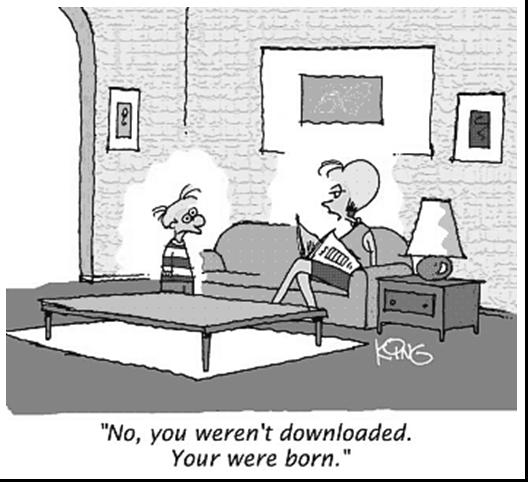
\includegraphics[width=.5\textwidth]{fig1.jpg}
\caption{A typical figure}
\label{fig:exampleFig1}
\end{figure}

\begin{figure}[ht]
\centering
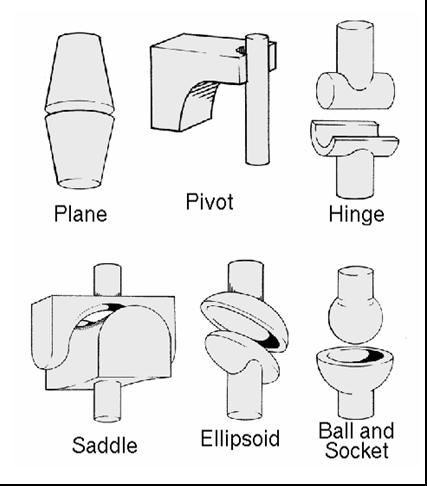
\includegraphics[width=.3\textwidth]{fig2.jpg}
\caption{This figure is an example of a figure caption taking more than one
  line and justified considering margins mentioned in Section~\ref{sec:figs}.}
\label{fig:exampleFig2}
\end{figure}

In tables, try to avoid the use of colored or shaded backgrounds, and avoid
thick, doubled, or unnecessary framing lines. When reporting empirical data,
do not use more decimal digits than warranted by their precision and
reproducibility. Table caption must be placed before the table (see Table 1)
and the font used must also be Helvetica, 10 point, boldface, with 6 points of
space before and after each caption.

\begin{table}[ht]
\centering
\caption{Variables to be considered on the evaluation of interaction
  techniques}
\label{tab:exTable1}
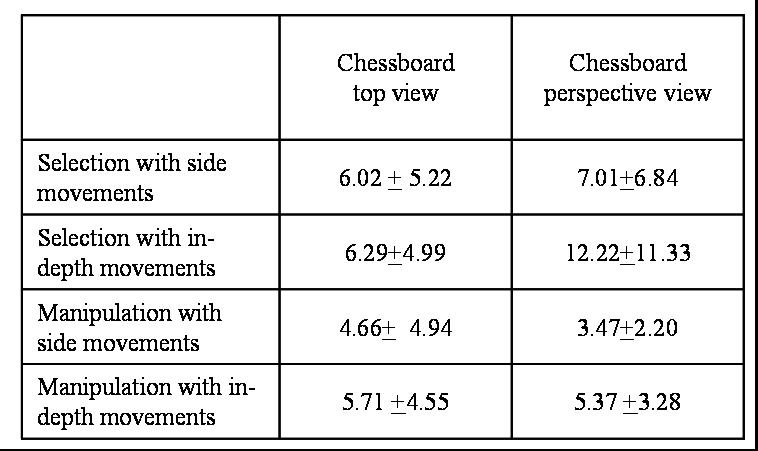
\includegraphics[width=.7\textwidth]{table.jpg}
\end{table}

\section{Images}

All images and illustrations should be in black-and-white, or gray tones,
excepting for the papers that will be electronically available (on CD-ROMs,
internet, etc.). The image resolution on paper should be about 600 dpi for
black-and-white images, and 150-300 dpi for grayscale images.  Do not include
images with excessive resolution, as they may take hours to print, without any
visible difference in the result. 

\section{References}

Bibliographic references must be unambiguous and uniform.  We recommend giving
the author names references in brackets, e.g. \cite{knuth:84},
\cite{boulic:91}, and \cite{smith:99}.

The references must be listed using 12 point font size, with 6 points of space
before each reference. The first line of each reference should not be
indented, while the subsequent should be indented by 0.5 cm.

\bibliographystyle{sbc}
\bibliography{sbc-template}

\end{document}
